\documentclass[border=4pt]{standalone}
\usepackage{tikz}
\begin{document}
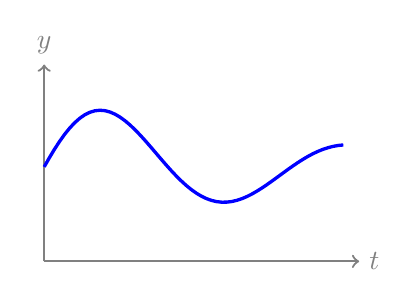
\begin{tikzpicture}[every node/.style={gray}]
  \draw[thick, ->, gray] (0,0) -- (4,0) node[right] {$t$};
  \draw[thick, ->, gray] (0,0) -- (0,2.5) node[above] {$y$};
  \draw[very thick, blue] plot[domain=0:3.8, samples=60] (\x, {1.2+0.9*sin(deg(2*\x))*exp(-0.3*\x)});
\end{tikzpicture}
\end{document}
